\documentclass[a4paper,14pt]{article}

\usepackage{amsmath,amsfonts,amssymb,amsthm,epsfig,epstopdf,titling,url,array}
\usepackage[utf8x]{inputenc}
\usepackage[russian]{babel}
%\usepackage[T2A]{fontenc}
\usepackage{amsmath,amssymb,amsthm,amscd,amsfonts,graphicx}
\usepackage[14pt]{extsizes}

\usepackage{cleveref}
\usepackage{tikz}
\usetikzlibrary{arrows,shapes,snakes,automata,backgrounds,petri}

\newcommand{\workflow}{\textit{workflow}}
\newenvironment{definition}[1]{
\hskip \labelsep {\bfseries #1} \it}

\newtheorem{theorem}{Теорема}
\newtheorem{lemma}{Лемма}
\newtheorem{corollary}{Вывод}



\begin{document}
\textwidth 15.5cm
\topmargin -1cm
\parindent 1cm
\textheight 24cm
\parskip 1.5mm



\section{Введение}
\subsection*{Цель работы}
Целью работы является построение модели workflow, ориентированного  на решение научно-инженерных задач в распределённой вычислительной среде. И разработка методов и инструментов анализа этой модели.
 Под инженерными и научными задачами в данном контексте мы понимаем 
мультидисциплинарные задачи в форме так называемых композитных приложений. В работе мы рассматриваем примеры задач обработки и анализа данных, например построения  суррогатных моделей , и задач многодисциплинарной оптимизации. Наиболее распространенным подходом к представлению таких композитных приложений является формализм потока работ, или workflow.

Под workflow подразумевается формальное представление (модель) некоторого процесса, включающее в себя:
\begin{enumerate}
\item[-] Описание операций, из которых состоит процесс.
\item[-] Описание исполнителей, которые выполняют указанные операции.
\item[-] Описание зависимостей между операциями, а именно :
\begin{enumerate}
\item[•] потоков управления, которые определяют последовательность выполнения операций 
\item[•] потоков данных, которые
определяют передачу информации между исполнителями.
\end{enumerate}
\end{enumerate}


Для выполнения задач, поставленных с помощью workflow, требуется система управления или исполнения( Workflow Managment system, WFMS)).Обычно WFMS состоит из набора программных
компонентов, предназначенных для:
\begin{enumerate}
\item[•] хранения и интерпретации описаний
процессов 
\item[•] создания и управления экземплярами запущенных процессов
\item[•] организации взаимодействия между участниками
процесса и внешними приложениями.
\end{enumerate}



\subsection*{Отличие научных workflow от бизнес-процессов}
  Исторически данный подход широко использовался для описания бизнес-процессов.Однако в данной работе мы рассматриваем научно-инженерные задачи. Приведём их некоторые характерные особенности:
 
\begin{enumerate}
\item[-] Научно-инженерные задачи требуют существенных вычислительных затрат.
\item[-] Научно-инженерные задачи работают с большими объёмами данных.
\item[-] Зачастую бывает  необходимо одинаковым образом обрабатывать разные наборы данные.
\item[-]  Ввиду перечисленных выше трёх пунктов, задачи могут быть ресурсоёмеими, поэтому имеет смысл использовать распределённую вычислительную среду.
\end{enumerate}

Традиционные WFMS, рассчитанные на работу с бизнес-процессами, в подавляющем большинстве не подходят для решения научных задач. Поэтому, требуется разработка новых, научных WFMS, с одной стороны опирающихся на сформировавшуюся workflow-методологию, а с другой стороны — специально рассчитанных на требования научных приложений.

\section{Обзор существующих моделей и подходов к представлению Workflow}

Свою работу мы начали с изучения уже существующих систем
\subsection*{Модели управления запуском Workflow}
  Все моделей управления workflow можно разделить на два класса: модели ориентированные на потоки управления(control-flows) и модели ориентированные на потоки данных(data-flows).  
  В первом случае(control-flow) явно задаётся порядок выполнения элементов workflow. К примеру, это позволяет естественным образом задавать циклы и условные переходы.
  Во втором случае (data-flow) явно задаются зависимости между данными, а система сама определяет последовательность выполнения.
  Так же существует гибридная модель управления, сочетающая оба эти принципа. Но всё равно, один из подходов является доминирующим. 
  
\subsection*{Представление Workflow}
За время существования методологии workflow возникло несколько различных подходов к их формальному описанию. Вот наиболее распространённые:
\begin{enumerate}
\item[•] Скриптовые языков.
 Скриптовые языки могут быть удобны пользователям(инженерам или исследователям), имеющим опыт программирования. Но не смотря на то , что  используемые  скрипты являются языками программирования высокого уровня , они не достаточно наглядны и интуитивны.
\item[•] Второй подход к описанию workflow - это использование ориентированных ациклических графов(DAG);
 Плюсы этого подхода - простота структуры и реализации.
  Но есть и недостатки. При таком подходе сложно описать процесс, имеющий итеративную природу, например задачу оптимизации. 
\item[•] Третьим подходом является использование сетей Петри.
 Сети Петри — это графический язык. Он
интуитивно понятен. К тому же сети Петри были хорошо исследованы и отличаются наличием большого числа методов анализа.
\end{enumerate}

В чистом виде перечисленные методы представления workflow не подходят для наших задач, и мы применяем некоторый гибридный подход.
 Как уже было сказано, в научных приложениях зачастую все необходимые действия сводятся к различным операциям над данными, и обычно в подобных процессах потоки управления и потоки данных совпадают. В следствии этого мы опираемся на модель потоков данных, т.е. data-flow.
 
 
\section{План работ}

\begin{figure}[here]
    \centering
    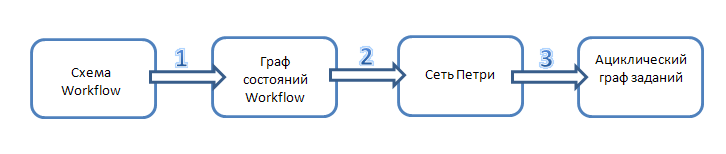
\includegraphics[width=\textwidth]{analys_plan.png}

    \label{img:opt_wf}
\end{figure}

 В нашей работе были сделаны следующие вещи:
\begin{enumerate}
\item Разработана и описана новая модель workflow.
\item Разработан и реализован алгоритм, моделирующий поведение модели. В результате работы этого алгоритма мы получаем граф всех достижимых состояний workflowю
\item Был предложен механизм анализа Этого графа состояний с целью выработки стратегии запуска в распределённой вычислительной среде.
\end{enumerate}
Рассмотрим эти этапы более подробно  
 
\section{Описание разрабатываемой модели Workflow}
\begin{figure}[here]
    \centering
    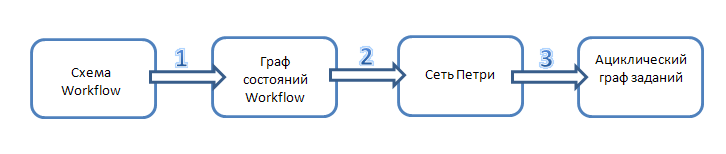
\includegraphics[width=\textwidth]{analys_plan.png}

    \label{img:opt_wf}
\end{figure}
Начнём с описания модели workflow.


Базовыми элементами нашей модели являются блоки и связи.
  Связи - это абстракция передачи данных, считаем, что данные между блоками передаются мгновенно и без потерь.
  Более того, в рассматриваемой модели мы абстрагируемся от типизации данных передаваемых между блоками, т.е. рассматриваем их как сигналы.
  
  Блок в нашей модели является единицей исполнения workflow,  реализующей некоторую задачу предметной области.Блок имеет интерфейс в виде входных и выходных портов. При это ключевой особенность модели является то, что блоки обладают нетривиальным поведением. Это поведение заключается в том, что в каждый момент модельного времени блок  декларирует наборы входных портов, необходимых для своего запуска. После того как одно из условий запуска было удовлетворено, т.е. получены данные на один из указанных наборов портов, блок выполняется и выдаёт данные в выходные порты. При это по завершению такого шага блок переопределяет условия следующего своего запуска.
  
Для того, чтобы пояснить суть блока в нашей модели, рассмотрим нетривиальный пример:

\begin{figure}[here]
    \centering
    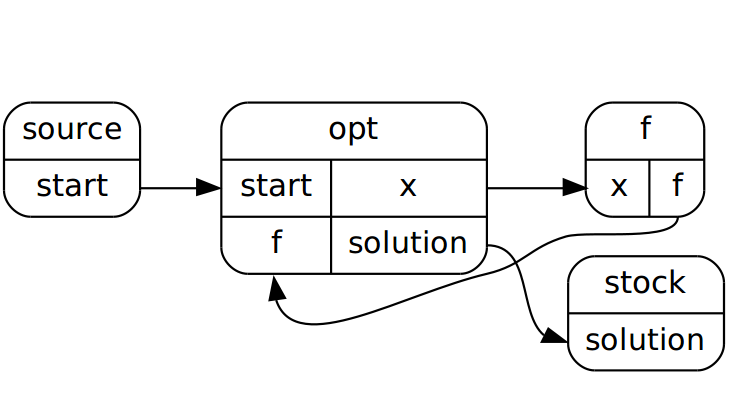
\includegraphics[width=0.5\textwidth]{optimization_workflow.png}
    \caption{Схема workflow для задачи оптимизации}
    \label{img:opt_wf}
\end{figure}


Данный workflow описывает задачу оптимизации.
Блок f - представляет тривиальный блок, считающий целевую функцию, всегда требующий данные на входной порт x  и всегда выписывающий данные в порт f.
Блок оптимизации уже не является тривиальным. В первый момент времени , он требует данные во входной порт start, далее итеративно выписывает данные в порт x, требую данные на входном порте f. И после того как оптимизация завершилась выдаёт данные с результатом уже в порт solution. При этом условием следующего запуска будет получение данных из порта start.


Таким образом, мы видим , что блок изменяет своё внутреннее состояние , сообщая системе условия, которые должны выполниться для его следующего запуска.



Для формального описания блока мы используем конечный недетерминированный автомат.

 К примеру, граф состояний оптимизирующего блока выглядит след образом:
\begin{figure}[here]
    \centering
    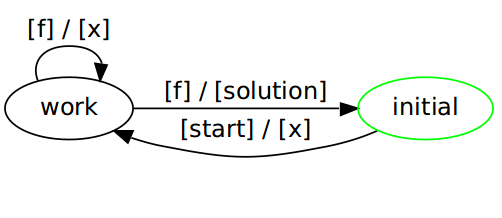
\includegraphics[width=0.5\textwidth]{optimizer_block.png}
    \caption{Граф состояний и переходов для оптимизирующего блока }
    \label{img:opt_wf}
\end{figure}

Где вершины графа - это состояния. А рёбра -  переходы. Подписи на рёбрах показывают , какие порты необходимы для осуществления перехода, и в какие порты будут выписаны данные.

Из начального состояния initial существует только один переход по порту start и выписка данных в порт x.  Из состояния work существует два возможных перехода: 
\begin{enumerate}
\item В себя же, поглощая данные из порта f  и выписывая в порт x.
\item Переход в начальное состояние с поглощением из f  и выписка данных в порт solution.
\end{enumerate}


Более строго блок описывается конечным недетерминированным автоматом, который задаёт:
\begin{enumerate}
\item[-] все возможные состояния блока
\item[-] набор входных и выходных портов
\item[-] некоторое выделенное начальное сосотояние
\item[-] все возможные переходы
\end{enumerate}
\begin{definition}{Определение: Конечный автомат блока} Конечным автоматом блока называется набор $M = (\Sigma, I, O, T, s_{0})$ , где
\begin{enumerate}
\item[-] $\Sigma$ -набор конечных состояния,
\item[-] $I$ - непустой набор доступных входных портов блока,
\item[-] $O$ - непустой набор доступных выходных портов блока,
\item[-] $I \bigcap O = \varnothing$ - 
\item[-] $s_{0} \in \Sigma$ - начальное состояние,
\item[-] $T: \Sigma \times (2^{I} \backslash \lbrace \varnothing \rbrace) \rightarrow  2^{\Sigma \times 2^{O}}$ отображение сопоставляющее каждому состоянию и набору входных портов набор состояний с соответствующим набором выходных портов.
\end{enumerate}
\end{definition}



\section{Анализ модели}
\begin{figure}[here]
    \centering
    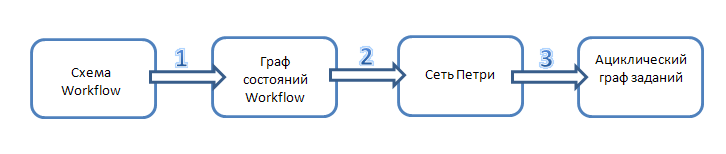
\includegraphics[width=\textwidth]{analys_plan.png}

    \label{img:opt_wf}
\end{figure}

 Перейдём к анализу описанной модели.
 Для анализа модели был разработан алгоритм, получающий на вход некоторый workflow и выдающий граф всех его достижимых состояний, который даёт исчерпывающую информацию о поведении workflow.
 Алгоритм по сути является волновым, при этом его особенностью является то, что при возникновении неоднозначности рассматриваются все варианты развития событий.
 
 
 Данный алгоритм так же позволяет обнаружить следующие ошибки , допущенные при составлении workflow:
 

Мы подразумеваем возможность асинхронной работы блоков на отдельных участках workflow. Следовательно то как и в многопоточных компьютерных программах возможно возникновение \textit{состояние гонки}(Race condition). 
В контексте нашей модели workflow состояние гонки бывает двух типов:
\begin{enumerate}
\item[•] Случай, когда на один входной порт блока приходят два сигнала одновременно.
\item[•] Когда на входные порты блока одновременно приходит такой набор сигналов, что существует неоднозначность запуска.

\end{enumerate}

Так же к ошибкам относятся  ситуации, когда на входных портах остаются данные, которые никогда не будут обработаны. Такие ситуации называются тупиками(deadlocks)

Наш алгоритм успешно детектирует данные ошибки до фактического запуска workflow, кот может длиться часами, днями, неделями.




\section{Анализа модели workflow}
\begin{figure}[here]
    \centering
    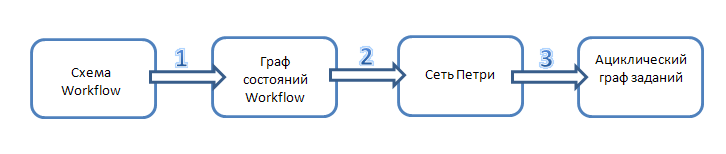
\includegraphics[width=\textwidth]{analys_plan.png}

    \label{img:opt_wf}
\end{figure}

После того, как был получен граф всех возможных состояний проделываем ряд преобразований с целью получить стратегию запуска данного workflow в распределённой вычислительной среде.
\subsection{Приведение к сети Петри}
Первым шагом является приведение графа всех достижимых состояний к виду сети Петри. Для этого мы сопоставляем каждому состоянию workflow одну или несколько позиций сети Петри, а каждому ребру графа один или несколько переходов., где каждый переход является запуском того или иного блока в определённом состоянии.


\subsection{Упрощение сети Петри}
Следующим шагом является избавление от циклов и условных переходов полученной сети Петри. Для этого мы доопределяем блоки вероятностями переходов из одного состояния в другое.
Это позволяет нам оценить среднее время работы подграфов, содержащих циклы и условные переходы и заменить их  эквивалентными по времени выполнения последовательностями выполняемых переходов.

После того, как были проделаны процедуры по устранению циклов и условных переходов, сеть Петри будет представляться только последовательными и параллельными участками. Позиции при такой структуре, могут быть соединены не более чем с двумя переходами. Удаляя все вершины графа, обозначающие позиции, и добавляя рёбра соединяющие смежные с этой позицией переходы, получим ациклический граф задач. 

\subsection{Выработка стратегии запуска}
Теперь, используя полученный граф задач стратегию запуска. Стратегией запуска мы называем распределение блоков по узлам. Т.е. требуется такое статическое распределение , что оценочное время выполнения workflow было минимальным при условии, что среднее значение показателя утилизации ресурсов было не меньше заданного уровня.

Для поиска такой стратегии использовался метод роя частиц.
Предложенный подход формирования стратегии запуска был опробован на множестве реальных и модельных задач и продемонстрировал разумные результаты.


\section{Итоги}

Подводя итоги,в работе было сделано следующее:
\begin{enumerate}
\item Разработана и описана модель Workflow
\item Разработан и реализован алгоритм анализа предложенной модели
\item Предложен подход к формировании стратегии запуска данной модели в распределённой вычислительной среде
\item Был разработан программный комплекс, реализующий всё выше перечисленное.
\item С помощью этого программного комплекса были поставлены эксперименты демонстрирующие жизнеспособность такого подхода.
\item  В дальнейшем планируется улучшение и доработка предложенных в работе подходов с целью улучшения качества распределения. 
\end{enumerate} 



%\subsection{Модифицированный волновой алгоритм}
%В работе был разработан алгоритм моделирования выполнения workflow для исследования поведения workflow и нахождения описанных ранее ошибок. Особенность этого алгоритма в том, что при возникновении неоднозначности рассматриваются все варианты развития событий.
%
%Мы считаем сценарий workflow корректным , если в нём невозможно возникновение состояния гонки. Т.е. порядок запуска блоков не зависит от времени работы любого из блоков, а только от распространения сигналов. И так как время работы блоков априори неизвестно, то примем, что время работы каждого блока фиксировано и равно некоторому значению T >0.
%
%Разработанный алгоритм последовательно, начиная из начального состояния, c шагом по времени T находит все достижимые уникальные состояния workflow и для каждого осуществляет проверку на возникновение состояний гонки. 
%Алгоритм останавливается, если была обнаружена ошибка или на новом шаге не было получено новых уникальных  состояний. 
%
%Состояние workflow в некоторый дискретный момент времени кратный T однозначно характеризуется состояниями каждого из блоков в составе анализируемого workflow в текующий момент времени и набором связей, по которым сигналы отправлены, но ещё не были поглощены.
%Начальным состоянием workflow будем называть то состояние в котором каждый блок находится в своём начальном состоянии, в соответствии с его конечным автоматом, и набор активных связей, состоит только из связей выходящих из блока Source.
%
%
%На основе получаемых в ходе работы алгоритма состояний workflow может быть построен ориентированный граф состояний workflow, где набор вершин - все найденные уникальные состояния, а ориентированные рёбра - переходы из одного состояния в другое за 1 шаг.

Полученный граф состояний отображает динамику работы workflow.

\begin{figure}[here]
    \centering
    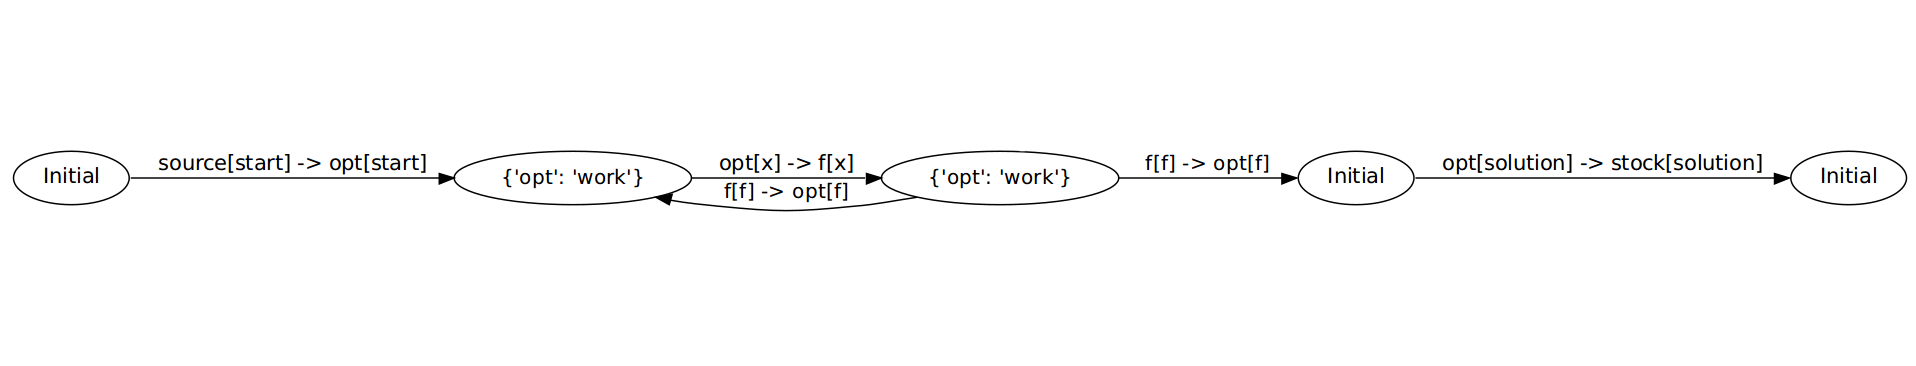
\includegraphics[width=\textwidth]{optimization_state_graph.png}
    \caption{Граф состояний и переходов для оптимизирующего блока }
    \label{img:opt_wf}
\end{figure}

%\subsection{Представление в виде сети Петри}
%При моделировании динамических систем, таких как workflow, с помощью сетей Петри используется нотация, при которой состояния системы  обозначаются позиции, а исполняемые задания - переходами.
%
%По определению состояние workflow несёт информацию о состоянии автомата и о доступных сигналах на входных портах для каждого блока системы в определённый дискретный момент времени. Для каждого ребра графа состояний, по начальной и конечной вершине, мы можем определить, какие блоки и в каких состояниях асинхронно выполнили работу за 1 шаг.
%
%Каждое состояние workflow, представляется набором из одного или нескольких положений сети Петри, число которых равняется числу блоков, с сигналами на входных портах. И каждое положение - характеризует информацию о доступных сигналах на  входных портах конкретного блока с конкретным текущим состоянием автомата при данном состоянии workflow.
%
% Соответственно, полученный граф состояний можно представить в виде сети Петри, путём сопоставления, каждому состоянию одной или нескольких позиций в контексте сетей Петри, а каждому ребру графа, соединяющему состояния, один и несколько переходов, соединяющих соответствующие позиции. 


\begin{figure}[here]
    \centering
    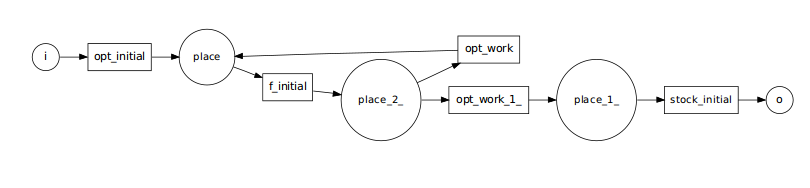
\includegraphics[width=0.8\textwidth]{optimization_petri_net.png}
    \caption{Граф состояний и переходов для оптимизирующего блока }
    \label{img:opt_wf}
\end{figure}



%\subsection{Планирование запуска }
%
%Задача построения стратегии запуска научно-инженерных workflow,как правило,включает в себя распределение заданий между доступными вычислительными ресурсами. Решение такой задачи обычно сводится к оптимизации функции затрат, зависящей от оценок времени работы заданий и производительности ресурсов. Более сложные планировщики, так же могут учитывать ещё и время, затрачиваемое на передачу данных между задачами. \\
%
%В силу того, что для нахождения оптимального решения задачи планирования должны быть рассмотрены все возможные варианты распределения заданий между ресурсами, задача планирования относится к классу NP-полных. Поэтому для нахождения около-оптимальных стратегии обычно используются эвристические подходы. Но получаемый результат в ходе применения таких подходов сильно зависит от точности используемых оценок времени работы заданий.
%
%Большинство существующих методов планирования применимы только к ациклическим ориентированным графам задач. Если же система представлена графом задач , содержащим циклы, то к ней применяют методы избавления от циклов.\\
%В подходе, представленном в работе, используя дополнительную эмпирическую информацию о вероятностях переходов, будем преобразовывать полученную сеть Петри, избавляясь от циклов и условных переходов, путём расчёта мат. ожидания количества срабатываний каждого перехода.
%
%
%После того, как были проделаны процедуры по устранению циклов и условных переходов, сеть Петри будет представляться только последовательными и параллельными участками. Позиции при такой структуре, могут быть соединены не более чем с двумя переходами. Удаляя все вершины графа, обозначающие позиции, и добавляя рёбра соединяющие смежные с этой позицией переходы, получим ациклический граф задач. Так же для каждого задания мы знаем усреднённое время требуемое для выполнения.
%
%Возвращаясь к поставленной задаче, мы хотим найти стратегию запуска workflow в распределённой вычислительной среде.
%Задача планирования (или нахождения стратегии запуска) workflow, может быть сформулирована в виде:
%
%\par "Найти такое статическое распределение блоков по узлам вычислительной сети из N допустимых узлов, что оценочное время выполнения всего workflow было минимальным при условии, что среднее значение показателя утилизации ресурсов было не меньше задаваемого уровня."
%
%Опишем некоторые ограничение, вводимые для упрощения поставленной задачи.
%\begin{enumerate}
%\item[•] Считаем , что блоки не переносимы с одного узла на другой.
%\item[•] На одном узле может быть запущено несколько блоков, но работать они могут только последовательно.
%\end{enumerate}
%
%
%
%




\end{document}